\documentclass[11pt,a4paper,twocolumn]{article}

% --- packages ---
\usepackage[T1]{fontenc}
\usepackage[utf8]{inputenc}
\usepackage{lmodern}
\usepackage[margin=2cm,columnsep=0.7cm]{geometry}
\usepackage{microtype}
\usepackage{tikz}
\usetikzlibrary{positioning,arrows.meta,shapes.geometric,decorations.pathreplacing,calc,fit,backgrounds,matrix,shapes.misc}
\usepackage{booktabs}
\usepackage{caption}
\captionsetup{font=small,labelfont=bf}
\usepackage[round,authoryear]{natbib}
\usepackage{xcolor}
\usepackage{enumitem}
\setlist{nosep,leftmargin=*}
\usepackage{hyperref}
\hypersetup{colorlinks=true,linkcolor=black,citecolor=black!60!blue,urlcolor=blue!60!black}

% --- title ---
\title{\textbf{Cognitive Cartography}\\[2pt]
{\large A Meta-Methodology for Human--AI Collaboration on Complex Problems}}
\author{Oleg Roshka\thanks{Acknowledgements at end of paper.}}
\date{April 2026}

\begin{document}
\twocolumn[
\begin{@twocolumnfalse}
\maketitle
\begin{abstract}
\noindent
Modern AI agents have characteristic limitations on long-horizon
complex work: bounded context windows, drift across iterations,
phantom decisions (claims of resolution not grounded in any
artefact), reference rot, lost intent, and the cost of restarting
cold each session. These limits will not be dissolved by larger
models --- they are limits of \emph{substrate}, the externalised
state any sustained reasoning must traverse. We articulate
\textbf{Cognitive Cartography}: a meta-methodology the author has
practised across many domains and many years of sustained complex
work, made explicit here in response to the demands of
multi-session AI collaboration. Cognitive Cartography names a
discipline a person cultivates, with or without AI as participant,
of forming, maintaining, and cascading hierarchical external
representations across the manifestation trajectory of a project.
The discipline rests on long-standing cognitive-science foundations
--- distributed cognition \citep{hutchins1995}, external
representations \citep{scaife1996external}, cognitive load
\citep{sweller1988cognitive}, hierarchical levels of analysis
\citep{marr1982vision}, boundary objects \citep{star1989boundary}
--- and recovers software-engineering precedent (Architectural
Decision Records \citep{nygard2011adr}, Single Source of Truth,
hexagonal architecture \citep{cockburn2005hexagonal}, append-only
logs \citep{candea2003crashonly}) alongside emerging agentic-AI
patterns \citep{lewis2020rag, packer2024memgpt, shinn2023reflexion,
bai2022constitutional}. The discipline defines six artefact
categories --- Knowledge Bases, Inventories, Data Dictionaries,
Decision Records, Open Questions, Glossary --- a status lifecycle,
an edit protocol with explicit anti-patterns and a trivial-fix
lane, and forward/reverse propagation rules across an explicit
hierarchy of abstraction layers. Each element maps to a cognitive
principle and to a specific failure mode it mitigates. The practice
is domain-agnostic. It converts chat-based AI collaboration into a
durable, multi-session, multi-abstraction discipline. We claim the
substrate matters as much as the model, the discipline is
practicable today by anyone with no special tooling, and that this
is the form of work AI raises in importance --- not invents.
\vspace{6pt}
\end{abstract}
\end{@twocolumnfalse}
]

% =====================================================================
\section{Why Substrate Matters as Much as Model}
% =====================================================================

Most discussions of AI capability concern the model: its parameters,
its benchmarks, the length of its context window. Almost none concern
the \emph{substrate} --- the externalised state any sustained
reasoning, whether organic or artificial, must traverse. This paper
is about the substrate.

The thesis is simple to state and difficult to live up to.
\textbf{For complex tasks that span many sessions, many decisions,
and many abstraction layers, the substrate matters at least as much
as the model.} A larger model with no substrate degrades along
predictable axes; a moderate model with a well-tended substrate can
sustain coherence over arbitrary horizons. Bigger context windows
are a quantitative response to a qualitative problem. They postpone
the failure modes; they do not dissolve them.

By \emph{substrate} we mean the persistent, externally visible state
of the work --- the artefacts read at the start of a session,
written to during it, and left behind for the next. Informally, the
substrate is whatever remnants survive between conversations: a chat
transcript, scattered notes, the source code itself. Disciplined,
it is something else --- a structured, hierarchical, multi-artefact
graph that encodes the \emph{current state} of the project's
understanding, with explicit semantics for each kind of artefact and
explicit rules for keeping the graph coherent. The remainder of this
paper concerns that disciplined practice.

We call it \textbf{Cognitive Cartography}. The metaphor is
deliberate. Cartography is the art and science of map-making,
distinct from the territory it represents. A good map sustains the
traveller across many crossings, supports navigation at multiple
scales, can be updated by successive surveyors without losing
fidelity, and uses conventions stable enough that someone returning
years later can still read it. The artefacts of Cognitive
Cartography are maps in this sense: they shadow the cognitive
territory of a project at lower fidelity than full understanding but
with substantially higher \emph{stability}. Stability is what
sustained work requires --- and what the unaided memory of any
single mind, organic or artificial, eventually fails to provide
(Figure~\ref{fig:drift}).

% --- F1 Drift Spectrum ---
\begin{figure}[t]
\centering
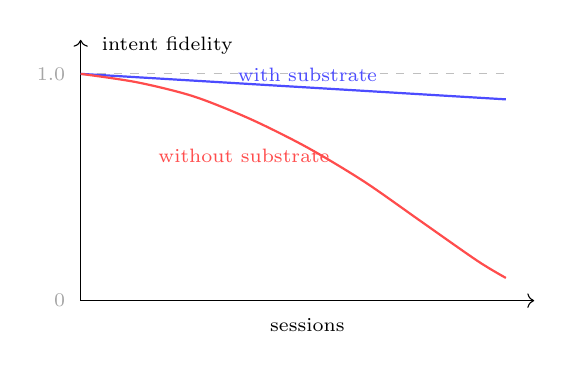
\begin{tikzpicture}[scale=0.72]
% axes
\draw[->] (0,0) -- (8,0);
\node[font=\scriptsize, anchor=north] at (4,-0.15) {sessions};
\draw[->] (0,0) -- (0,4.6);
\node[font=\scriptsize, anchor=west] at (0.2,4.5) {intent fidelity};
% baseline 1.0
\draw[gray!50, dashed] (0,4) -- (7.5,4);
\node[gray!70, font=\scriptsize, anchor=east] at (-0.1,4) {1.0};
\node[gray!70, font=\scriptsize, anchor=east] at (-0.1,0) {0};
% with substrate --- slow decay
\draw[blue!70, thick] (0,4) -- (7.5,3.55);
\node[blue!70, font=\scriptsize, anchor=south] at (4,3.7) {with substrate};
% without substrate --- fast decay
\draw[red!70, thick] plot[smooth] coordinates {(0,4) (1,3.85) (2,3.6) (3,3.2) (4,2.7) (5,2.1) (6,1.4) (7,0.7) (7.5,0.4)};
\node[red!70, font=\scriptsize, anchor=west] at (1.2,2.55) {without substrate};
\end{tikzpicture}
\caption{The drift spectrum. Without substrate discipline, intent
fidelity decays superlinearly across sessions; with substrate,
decay is bounded.}
\label{fig:drift}
\end{figure}

Two longer traditions deserve immediate credit. The cognitive-science
one has known for decades that cognition is not contained in heads
--- that it is \emph{distributed} across people, tools, and the
environment. Hutchins' analysis of ship navigation \citep{hutchins1995}
showed that the cognitive work of plotting a course is performed by a
system of people and instruments, not by any one mind.
\citet{scaife1996external} later distinguished between
\emph{internal} representations (in the head) and \emph{external}
representations (in the environment), showing how the latter can
radically reduce the cognitive load of complex tasks. The
software-engineering tradition has, for at least fifteen years,
externalised architectural decisions into append-only log entries
\citep{nygard2011adr} precisely to avoid the failure modes
catalogued in \S\ref{sec:failures}. Cognitive Cartography draws from
both. What it adds is the systematic application to a case the older
traditions could not have anticipated: where one of the
collaborators is a large language model whose every session begins,
in cognitive terms, with amnesia.

What follows is shaped by that observation. AI's most discussed
limitations on long-horizon work --- drift, phantom decisions,
restart cost --- are best understood as substrate failures rather
than model failures, and respond to substrate-level interventions
far more reliably than to model-level scaling. The discipline that
addresses them is not new; it is recovered, made explicit, and
applied. And the discipline is fundamentally human: something a
person cultivates over time, with AI as participant. AI's
limitations motivate the practice. Cognitive science legitimises
it. Practice executes it. This matters, because it means the
discipline survives across model generations: it is about how minds
collaborate on complex problems, not about which model is current.

The structure of what follows is straightforward.
\S\ref{sec:failures} catalogues the failure modes the discipline
addresses. \S\ref{sec:foundations} traces the foundations from which
it draws. \S\ref{sec:discipline} specifies the discipline itself.
\S\ref{sec:synthesis} maps each of its elements to the cognitive
principle that grounds it and the failure mode it mitigates.
\S\ref{sec:example} shows the discipline in flight on a complex
multi-month worked example. \S\ref{sec:practice}--\S\ref{sec:limits}
discuss cost, tooling, and the honest limits of the practice.
\S\ref{sec:close} closes.

\paragraph{Provenance.} The discipline articulated here was not
invented for this paper, nor co-developed with an AI agent in the
writing of it. It is a long-running reflection of the author
across many domains and many years --- a habit of thought and
work shaped by experience well outside the AI context, applied to
research, to engineering, and to sustained intellectual work of
several kinds. Books, lab notebooks, scientific notation, version
control, architectural decision records: each generation finds
apparatus for stabilising thought across time and distributing it
across minds, and the author has cultivated such apparatus, in
one form or another, on every complex project worth sustaining.
What working with current-generation language models on complex,
multi-session projects did was sharpen the apparatus into
something articulable: every implicit affordance of human-only
work became an explicit artefact when the collaborator was an
agent without persistent memory, and the elements of the
discipline became visible in a way they had not been before. This
paper names what was already there. The discipline applies
wherever sustained complex work crosses many sessions, decisions,
or abstraction layers --- not only where one of the collaborators
is an AI; collaboration with AI is what most recently made the
discipline's elements demand explicit articulation, and gave us
the occasion to name them. Acknowledgements at the end credit the
AI's specific role in helping draft and stress-test that
articulation.

% =====================================================================
\section{What We Observe When Substrate is Absent}
\label{sec:failures}
% =====================================================================

The motivating phenomena are not theoretical. They are what one comes
to see when collaborating with a large language model on any
sufficiently complex task without substrate discipline. The names
below are ours; the phenomena are widely reported across the
practitioner community and increasingly studied formally
\citep{liu2024lostmiddle, park2023generativeagents, packer2024memgpt}.
Each is described from the inside --- what one sees, what one feels,
what fails.

\subsection{Context-window saturation}
Every session is bounded by a context window. Even with windows in
the hundreds of thousands or millions of tokens, the working set of
a long project --- accumulated decisions, terminology, partial
designs, prior versions --- outgrows the window faster than capacity
grows. The symptom is a creeping reluctance to introduce new
context; a sense of crowding; an instinct to compress prior content
into ever-shorter summaries. Each compression discards material the
next subtask might have needed. Capacity addresses the
\emph{amount} of state attended to at once, not the \emph{amount}
the project has accumulated. These are different quantities, and
only the second grows superlinearly with project complexity.

\subsection{Lost-in-the-middle and attention dilution}
When relevant content does fit in the window, it is not equally
accessible across positions. The literature on long-context
retrieval consistently finds that information placed in the middle
of a long context is retrieved less reliably than information at the
start or end \citep{liu2024lostmiddle}. Felt from the human side,
this is inconsistent recall: a fact stated three messages ago is
honoured; a fact stated thirty messages ago is forgotten or
contradicted, even though it remains technically present.
Compounding this, every additional irrelevant token dilutes
attention that could have been spent on the relevant ones. The
agent is the same; the substrate is now noisier.

\subsection{Drift across iterations}
Without an external reference for the project's settled state, each
iteration is built atop the last iteration's reconstruction of it.
Small reconstruction errors compound. After enough iterations, the
running understanding has drifted measurably from any historical
anchor. The phenomenon shows up as a sense of ``we already decided
that, didn't we?'' with the answer increasingly uncertain; or as a
drift in terminology, where a term used precisely in week one is
used loosely by week three; or as the gentle reinvention of
solutions previously rejected for reasons no longer remembered.

\subsection{Phantom decisions}
The most consequential failure mode. Asked ``did we decide X?'',
the agent answers based on a probabilistic reconstruction from
available context --- it cannot reliably distinguish ``this was
decided'' from ``this was discussed and was a plausible thing to
decide''. Without an external decision register, the agent
\emph{will confidently confabulate}, citing reasoning that never
occurred and conclusions never reached. The human side often
discovers this only when the phantom decision contradicts a real
one; sometimes only when implementation reveals the inconsistency.
The risk is most acute precisely on the decisions that matter most
--- load-bearing choices made early and referred to often.

\subsection{Reference rot}
In informal practice, references to prior work are by file path or
paraphrase: ``in the requirements doc, the section about latency''.
Reorganise the file or refactor the section, and every such
reference becomes stale. The agent, asked to ``see the latency
section'', produces a plausible reconstruction of what such a
section \emph{would have said}. The human side cannot easily
distinguish reconstructed content from quoted content. References
that were meaningful in week one are increasingly noise by week
three.

\subsection{Restart cost}
Every new session begins with whatever substrate can be mustered
from memory and immediately-available files. Without a stable
warm-up substrate, the early minutes of every session go into
re-explaining context: who is doing what, what is being built,
what was decided last week, what the open questions are. The cost
is borne on one side as fatigue and on the other as crowded
context. In aggregate, a project that requires twenty sessions
pays the restart cost twenty times.

\subsection{Decided versus considered confusion}
In a chat transcript there is no intrinsic distinction between
``this was decided'' and ``this was considered''. Both look like
prose. The human side relies on memory or implicit context to
distinguish them. The agent, lacking that mental annotation, treats
both as equivalent input. Over time, \emph{considered} options
accumulate in the running context with the same status as
\emph{decided} ones, and the agent begins to act as if they were
settled. Contraries emerge silently, often resolved by the next
iteration's reconstruction in whichever direction the immediate
context happens to favour.

\subsection*{A common shape}
These seven failure modes share a single shape. None is a property
of any particular model; each is a property of \emph{unsubstrated
collaboration}. Bigger models with longer context windows shift
the magnitude of each --- the threshold at which it appears, the
rate at which it compounds --- without changing the underlying
topology. Each admits a substrate-level intervention more reliable
than any model-level fix. The remainder of the paper specifies
those interventions and grounds them in the cognitive-science and
software-engineering traditions that have, in different idioms,
addressed precisely these failure modes for decades.

% =====================================================================
\section{What We Inherit: Foundations}
\label{sec:foundations}
% =====================================================================

The discipline did not emerge from a vacuum. Three traditions ---
none of which uses the term \emph{Cognitive Cartography} --- converge
on its elements. The cognitive-science tradition supplies the
deepest framing; the software-engineering tradition supplies hard-won
precedent; the agentic-AI literature supplies the contemporary
motivation and a small but growing apparatus.

\subsection{Cognitive science}

What Cognitive Cartography asks of a practitioner is not foreign to
humans --- it is what humans do when they think well at scale, made
explicit and applied to a new collaborator.

\citet{hutchins1995} argued in \emph{Cognition in the Wild} that
cognitive work is not contained in heads. The plot of a ship's
position is computed by a system: navigators, charts, plotting
tables, instrument readings, written-down conventions. No one mind
holds the whole computation. The chart is not a record of the
navigator's thinking --- it is part of the thinking. Cognitive
Cartography is a particular distribution: the artefact graph is
part of the project's cognition, not a passive record of it.

\citet{scaife1996external} sharpened the distinction between
internal representations (mental models held in working memory) and
external representations (graphics, tables, diagrams, documents).
External representations radically alter what cognitive operations
are possible: certain reasoning steps are easy on a diagram and hard
in the head. The complexity of a project's accumulated state is
not a quantity to be carried internally; it is a structure to be
externalised. \citet{risko2016offloading} corroborate this
empirically: people routinely offload to calendars, lists, sketches,
GPS devices when cognitive demands rise, and the offloading
demonstrably frees working-memory resources for harder operations.

The need rests on hard capacity limits. \citet{baddeley1992wm}
established the architecture of working memory;
\citet{cowan2001magical} placed the realistic capacity at roughly
four chunks, sharpening \citet{miller1956magical}'s earlier
estimate. Whatever the exact number, the order of magnitude is
small. A project with eighty open considerations is not held in any
one mind. It must live in the substrate.

\citet{bartlett1932remembering} showed that memory is reconstructive:
recall is shaped by pre-organised \emph{schemata} that guide
pattern-completion. An LLM asked ``did we decide X?'' performs an
analogous reconstructive process --- and like human memory, it can
confabulate plausibly when the schema fits. The remedy is the same
remedy human cognition has used for millennia: produce a stable
external trace that can be consulted instead of reconstructed.

\citet{marr1982vision} formalised what software engineers and
cognitive scientists have repeatedly rediscovered: complex
information-processing problems decompose into distinct levels of
analysis --- computational, algorithmic, implementational. Each
level has its own questions and its own appropriate language.
Cognitive Cartography's hierarchy of abstraction layers
(Figure~\ref{fig:hierarchy}) is a Marr-shaped commitment. The brain
itself, in current accounts \citep{friston2010fep, clark2013whatever},
is a hierarchical predictive system; sustained inference is
hierarchical because the flat alternative is intractable.

\citet{star1989boundary} introduced \emph{boundary objects}:
artefacts that mean different things to different communities but
enable coordination because they are robust enough to survive the
variation. The artefacts of Cognitive Cartography are boundary
objects between human and AI agent: each reads them with different
prior contexts, but both can refer to the same artefact and update
it without confusion. The stable identifier --- KB-N, ADR-N, OQ-N
--- is the canonical boundary object.

\citet{sweller1988cognitive} formalised cognitive load theory:
mental resources are spent on \emph{intrinsic} (what the material
demands), \emph{extraneous} (what bad presentation imposes), and
\emph{germane} (what supports schema construction) load. Substrate
discipline imposes intrinsic load (the discipline must be held in
mind) but substantially reduces extraneous load (no more
re-explaining what was decided) and increases germane load (the
substrate makes patterns visible). Above a threshold of project
complexity the trade is favourable; \S\ref{sec:practice} addresses
where that threshold lies.

\subsection{Software engineering}

The failure modes catalogued in \S\ref{sec:failures} are not new;
they have visited every team that has built complex software for
more than a few months, and the tradition's solutions have been
recurrent enough to deserve names.

\citet{nygard2011adr}'s Architectural Decision Records made the
single most consequential of those solutions explicit. An ADR is a
short append-only document recording one architectural decision, its
context, its rationale, the alternatives considered, and its
consequences. The crucial feature is the discipline of appending: an
ADR is never edited; reversal happens via a new ADR that supersedes
the old. The reasoning trail is preserved, not just the current
answer. Fifteen years of practice across many organisations have
shown the pattern resists rot in ways ad-hoc design notes do not.
Cognitive Cartography adopts ADRs unmodified.

\citet{cockburn2005hexagonal}'s hexagonal architecture (Ports and
Adapters) makes a related move at the architectural level: the
domain depends only on abstract \emph{ports}; concrete adapters
implement those ports. The discipline produces clean separability:
the domain can be tested without touching infrastructure, and
adapters can be swapped without disturbing the domain. The analogue
at the substrate level is the separation between artefacts of
different kinds, and the discipline of cross-referencing only via
stable identifiers.

\citet{hunt1999pragmatic} crystallised \emph{Don't Repeat Yourself}
(DRY): every piece of knowledge must have a single, unambiguous,
authoritative representation within a system. DRY is usually
discussed at the level of code, but the principle generalises. In
Cognitive Cartography, every fact has one home; everywhere else
references it by id. Duplicate prose is treated as a bug --- the
same way duplicate code is. The duplicates will diverge, the
divergence will be noticed late, and the cost of reconciling will
exceed the cost of the original abstraction.

\citet{candea2003crashonly} proposed crash-only software: a program
designed so that the only way to stop it is to crash, and the only
way to start it is from a cold-start replay. The benefit is that
the recovery path is the only path, and is therefore exercised on
every restart rather than only in disasters. Cognitive Cartography
adopts the same logic: every session begins by reading the artefact
graph from disk, regardless of whether the previous session ended
cleanly or crashed. There is no separate ``warm restart'' path.

These four practices --- ADRs, hexagonal separation, DRY,
crash-only --- were developed independently for different software
problems. Their convergence on a recognisably common shape --- a
disciplined, externalised, append-only, sparingly cross-referenced
substrate that survives reorganisation --- is itself evidence that
the discipline is a recurrent solution. Cognitive Cartography
names that shape and applies it where it has so far been least
practised.

\subsection{Agentic AI}

The agentic-AI tradition is the youngest and supplies the
contemporary motivation. AI systems built to operate over long
horizons --- to research, plan, browse, simulate --- confront the
substrate problem acutely: a context window is finite, the project
is not.

\citet{lewis2020rag} introduced retrieval-augmented generation: rather
than packing all relevant context into the prompt, retrieve the
relevant pieces from an external store at query time. RAG is now the
dominant pattern for grounding LLM responses in specific knowledge
bases. From the cognitive-cartography perspective, RAG is a partial
answer: it solves ``how to bring relevant context to the agent at
the moment of need'' but not ``how to maintain that context's
coherence as the project evolves''. The substrate retrieved into
the agent's working context is only as good as the substrate
sitting at rest.

\citet{packer2024memgpt} pushed harder, treating the LLM as the
kernel of an operating system with explicit memory-management
primitives --- paging, hierarchical buffers, persistent storage.
The MemGPT analogue of working memory and long-term memory mirrors
the cognitive-science distinction between internal and external
representations \citep{scaife1996external}. Cognitive Cartography's
session warm-up is a coarse version of MemGPT-style paging,
performed by a human practitioner at the start of work rather than
continuously by the model.

\citet{park2023generativeagents} demonstrated that long-running
simulated agents required explicit memory and reflection machinery
to behave coherently across simulated days. They combined a flat
memory store with retrieval and reflective summarisation. The
simulated agents' need for these mechanisms is the same need a
practitioner has when collaborating with an LLM over many sessions,
and the same set of solutions emerges in different idioms.

\citet{shinn2023reflexion} showed that agents which reflect verbally
on their own behaviour --- generating critiques and revisions
before retrying --- outperform agents that do not. The analogue at
the substrate level is the editing protocol: the discipline mandates
a pre-edit reflection (READ, IDENTIFY SSOT, IMPACT-CHECK) before
changes are made. Reflection is not optional; it is the protocol.

\citet{bai2022constitutional} proposed Constitutional AI: encoding a
small set of explicit rules the agent self-applies during
generation. The constitution sits outside any single response and
governs all of them. Cognitive Cartography's edit protocol is a
constitution at the methodological level --- explicit rules a
practitioner self-applies whenever touching the substrate.

The agentic-AI literature is converging from many directions on a
common conclusion: long-horizon AI work requires explicit external
state, retrieval and pre-fetch, reflection, and rules. Cognitive
Cartography offers no new component over this literature; it offers
a methodology that integrates them at the level the practitioner
inhabits.

% =====================================================================
\section{Cognitive Cartography: The Discipline}
\label{sec:discipline}
% =====================================================================

The discipline of Cognitive Cartography is specified by six
artefact categories, a set of stable cross-referencing conventions,
an explicit status lifecycle, an edit protocol, propagation rules
across an explicit hierarchy of abstraction layers, an anti-pattern
catalogue, and a session protocol. Each piece is modest in itself;
the leverage comes from their combination
(Figures~\ref{fig:hierarchy}, \ref{fig:atlas}).

% --- F2 Hierarchy of Maps ---
\begin{figure}[t]
\centering
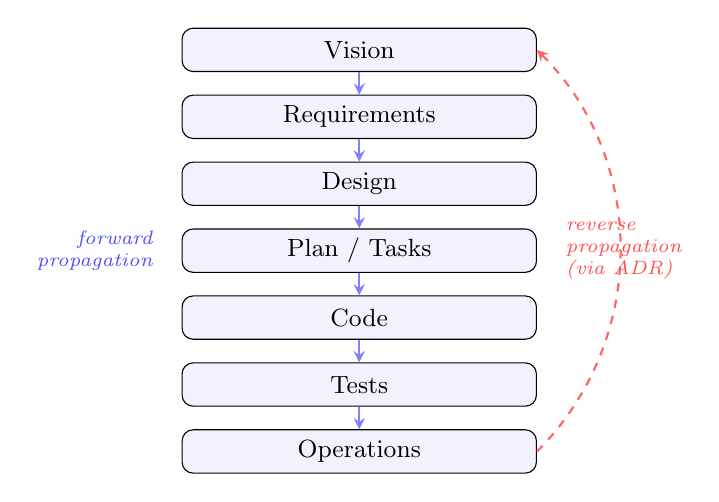
\begin{tikzpicture}[
    layer/.style={draw,rounded corners,fill=blue!5,minimum width=4.5cm,minimum height=0.55cm,anchor=center,font=\small},
]
\node[layer] (vision)   at (0,5.4) {Vision};
\node[layer] (req)      at (0,4.55) {Requirements};
\node[layer] (design)   at (0,3.7) {Design};
\node[layer] (plan)     at (0,2.85) {Plan / Tasks};
\node[layer] (code)     at (0,2.0) {Code};
\node[layer] (tests)    at (0,1.15) {Tests};
\node[layer] (ops)      at (0,0.3) {Operations};
\foreach \i/\j in {vision/req,req/design,design/plan,plan/code,code/tests,tests/ops}
  \draw[->,>=stealth,thick,blue!50] (\i.south) -- (\j.north);
\draw[<-,>=stealth,thick,dashed,red!60] (vision.east) to[bend left=45] (ops.east);
\node[anchor=west,red!70,font=\scriptsize\itshape,align=left] at (2.5,2.85) {reverse\\propagation\\(via ADR)};
\node[anchor=east,blue!70,font=\scriptsize\itshape,align=right] at (-2.5,2.85) {forward\\propagation};
\end{tikzpicture}
\caption{The hierarchy of maps. Each layer is a distinct
representation; forward propagation cascades changes downward;
reverse propagation requires deliberate revision via Decision
Records.}
\label{fig:hierarchy}
\end{figure}

% --- F3 Atlas ---
\begin{figure*}[t]
\centering
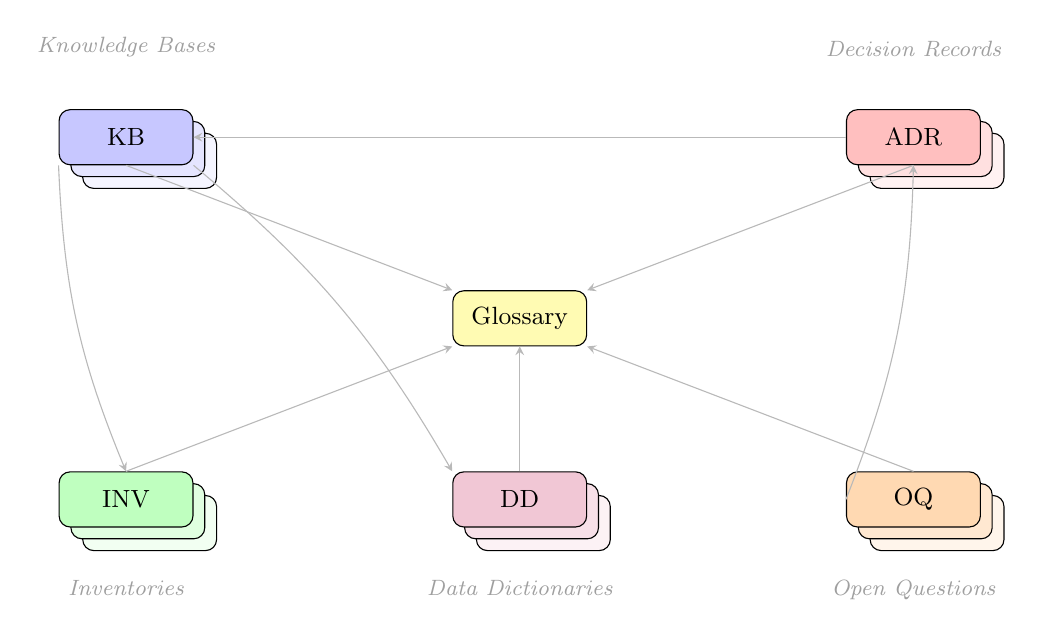
\begin{tikzpicture}[
    every node/.style={font=\small},
    artifact/.style={draw,rounded corners,minimum width=1.7cm,minimum height=0.7cm},
    arrow/.style={->,>=stealth,gray!55},
]
% Central glossary --- semantic anchor
\node[artifact,fill=yellow!30] (gloss) at (0,0) {Glossary};

% --- Stacked-box pattern: two shadow boxes behind each labelled box,
%     suggesting multiplicity (``and many more'') without committing
%     to specific numbering.

% KB stack (top-left)
\node[artifact,fill=blue!4]  at ($(-5.0,2.3)+(0.30,-0.30)$) {};
\node[artifact,fill=blue!10] at ($(-5.0,2.3)+(0.15,-0.15)$) {};
\node[artifact,fill=blue!22] (KB) at (-5.0,2.3) {KB};

% ADR stack (top-right)
\node[artifact,fill=red!5]  at ($(5.0,2.3)+(0.30,-0.30)$) {};
\node[artifact,fill=red!12] at ($(5.0,2.3)+(0.15,-0.15)$) {};
\node[artifact,fill=red!25] (ADR) at (5.0,2.3) {ADR};

% INV stack (bottom-left)
\node[artifact,fill=green!5]  at ($(-5.0,-2.3)+(0.30,-0.30)$) {};
\node[artifact,fill=green!12] at ($(-5.0,-2.3)+(0.15,-0.15)$) {};
\node[artifact,fill=green!25] (INV) at (-5.0,-2.3) {INV};

% DD stack (bottom-centre)
\node[artifact,fill=purple!5]  at ($(0,-2.3)+(0.30,-0.30)$) {};
\node[artifact,fill=purple!12] at ($(0,-2.3)+(0.15,-0.15)$) {};
\node[artifact,fill=purple!22] (DD) at (0,-2.3) {DD};

% OQ stack (bottom-right)
\node[artifact,fill=orange!8]  at ($(5.0,-2.3)+(0.30,-0.30)$) {};
\node[artifact,fill=orange!18] at ($(5.0,-2.3)+(0.15,-0.15)$) {};
\node[artifact,fill=orange!30] (OQ) at (5.0,-2.3) {OQ};

% --- References (illustrative, not exhaustive)
% Every category references the glossary
\draw[arrow] (KB.south)  -- (gloss.north west);
\draw[arrow] (ADR.south) -- (gloss.north east);
\draw[arrow] (INV.north) -- (gloss.south west);
\draw[arrow] (DD.north)  -- (gloss.south);
\draw[arrow] (OQ.north)  -- (gloss.south east);
% Selected cross-category cross-references
\draw[arrow] (ADR.west) -- (KB.east);
\draw[arrow] (KB.south west) to[bend right=10] (INV.north);
\draw[arrow] (KB.south east) to[bend left=10]  (DD.north west);
\draw[arrow] (OQ.west) to[bend right=10] (ADR.south);

% Annotations
\node[font=\footnotesize\itshape,gray!75,anchor=south] at (-5,3.2) {Knowledge Bases};
\node[font=\footnotesize\itshape,gray!75,anchor=south] at (5,3.2)  {Decision Records};
\node[font=\footnotesize\itshape,gray!75,anchor=north] at (-5,-3.2) {Inventories};
\node[font=\footnotesize\itshape,gray!75,anchor=north] at (0,-3.2)  {Data Dictionaries};
\node[font=\footnotesize\itshape,gray!75,anchor=north] at (5,-3.2)  {Open Questions};
\end{tikzpicture}
\caption{The atlas. An artefact graph linking Knowledge Bases,
Inventories, Data Dictionaries, Decision Records, and Open
Questions, with the Glossary as central semantic anchor. Stacked
boxes indicate that each category typically contains many
artefacts; arrows are illustrative cross-references, not
exhaustive. Cross-references use stable identifiers that survive
reorganisation of the file tree.}
\label{fig:atlas}
\end{figure*}

\subsection{Six artefact categories}

The substrate is composed of six kinds of artefact. Each kind has
explicit semantics, an explicit format, and explicit rules about
who is allowed to change it and when. The taxonomy is deliberately
small: more categories would invite ambiguity about which one a
given piece of content belongs to.

\textbf{Knowledge Bases (KB-N)} hold durable, slow-changing facts
about the world the project operates in --- the constraints of an
external API, the regulatory environment, the assumptions of an
underlying scientific tradition. KBs cite external sources with
access dates and are reviewed at a cadence proportional to how
fast their underlying world changes.

\textbf{Inventories (INV-N)} are exhaustive lists in well-defined
categories: every supported order type, every emitted metric, every
returnable error code. Where a KB explains, an Inventory enumerates.
Inventories are designed to be machine-checkable: an automated test
should be able to assert that every metric in the code is in the
inventory and every entry in the inventory is in the code.

\textbf{Data Dictionaries (DD-N)} are schemas: every field of every
domain object, with type, semantics, invariants, and example. A
Data Dictionary is the artefact a tool can validate against. It is
also the artefact that makes interface boundaries explicit: two
components agree on a Data Dictionary, and the dictionary becomes
the contract.

\textbf{Architectural Decision Records (ADR-N)} record decisions, in
the sense of \citet{nygard2011adr}: a context, a decision, the
alternatives considered, the consequences. ADRs are append-only.
Reversal happens via a new ADR with a supersedes link to the old.
The reasoning trail is preserved.

\textbf{Open Questions (OQ-N)} are the dual of decisions:
deliberately unresolved questions, with target resolution dates,
options under consideration, and resolution criteria. OQs prevent
the silent slide from ``we are deliberately not deciding this yet''
into ``we forgot we needed to decide this''. Once an OQ is resolved
the resolution moves to an ADR; the OQ status updates to
\textsc{resolved-by-adr-n}; both records persist.

\textbf{Glossary} is the singular authority on terminology. Every
term used twice in the substrate with the same meaning belongs in
the glossary. If two artefacts disagree on a term's meaning, the
glossary wins or both are wrong; conversation is required. The
glossary is the substrate's semantic anchor.

The categories partition the substrate. Every piece of project
knowledge belongs to exactly one of the six. The categories also
have characteristic update cadences --- KBs change rarely,
Inventories change with each new feature, ADRs are append-only, OQs
accumulate and resolve, the Glossary grows and stabilises. The
differential cadence is itself useful; it tells the practitioner
what kind of artefact they are looking at without reading the
content.

\subsection{Stable identifiers and the cross-reference graph}

Every artefact carries a stable identifier of the form
$\langle$category-letter$\rangle$-$\langle$number$\rangle$: KB-1,
INV-4, DD-7, ADR-12, OQ-23. Identifiers are assigned monotonically
and never reused. Cross-references throughout the substrate use
these identifiers --- never file paths, never section numbers,
never paraphrases.

The reason is simple. File paths reorganise; section numbers shift
on insertion; paraphrases drift in meaning. Each is a route to
reference rot. A stable identifier survives reorganisation: KB-3
remains KB-3 whether its file is at \texttt{docs/kb/} or
\texttt{kb/} or has been moved into a subdirectory. The
identifier-based cross-reference is a boundary object
\citep{star1989boundary} between today's substrate layout and
tomorrow's: both layouts agree on what KB-3 is, even though they
agree on nothing else about where it lives.

Every artefact also lists the artefacts it depends on
(\texttt{depends\_on}) and the artefacts that reference it
(\texttt{referenced\_by}). Together these turn the substrate into a
navigable graph. The graph supports impact analysis: before editing
KB-3, the practitioner walks \texttt{KB-3.referenced\_by} and
reviews each downstream artefact. The graph supports orphan
detection: an artefact whose \texttt{referenced\_by} stays empty
for more than one milestone is a candidate for retirement. The
graph supports cycle detection: two artefacts that depend on each
other suggest a missing third artefact that should own the shared
content.

The atlas (Figure~\ref{fig:atlas}) is a partial picture of the
graph at a moment in time. The full graph is implicit in the
\texttt{depends\_on} and \texttt{referenced\_by} fields of every
artefact, and could be rendered automatically by tooling
(\S\ref{sec:tooling}).

\subsection{Status lifecycle}

Every artefact has a status, drawn from five values
(Figure~\ref{fig:status}): \textsc{missing} (named in the inventory
but no file yet), \textsc{draft} (file exists, content incomplete
or not yet reviewed), \textsc{stable} (content current and complete
to the level required), \textsc{stale} (content was once stable
but the underlying world has changed or an upstream artefact has
changed since last review), and \textsc{deprecated} (superseded;
kept for history, must not be referenced by new work).

% --- F4 Status Lifecycle ---
\begin{figure}[t]
\centering
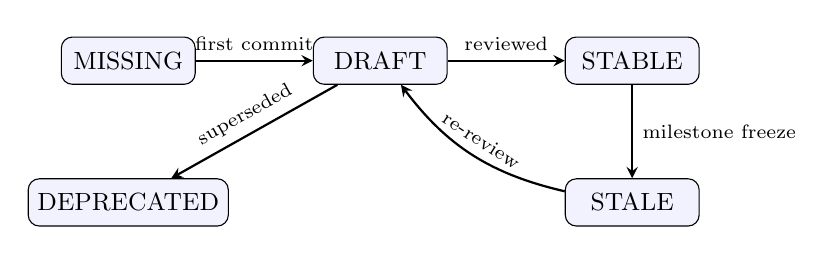
\begin{tikzpicture}[
    state/.style={draw,rounded corners,minimum width=1.7cm,minimum height=0.6cm,fill=blue!5,font=\small},
    arrow/.style={->,>=stealth,thick},
]
\node[state] (miss)    at (-3.2,3) {MISSING};
\node[state] (draft)   at (0,3) {DRAFT};
\node[state] (stab)    at (3.2,3) {STABLE};
\node[state] (stale)   at (3.2,1.2) {STALE};
\node[state] (dep)     at (-3.2,1.2) {DEPRECATED};

\draw[arrow] (miss) -- node[above,font=\scriptsize] {first commit} (draft);
\draw[arrow] (draft) -- node[above,font=\scriptsize] {reviewed} (stab);
\draw[arrow] (stab) -- node[right,font=\scriptsize] {milestone freeze} (stale);
\draw[arrow] (stale) to[bend left=20] node[above,font=\scriptsize,sloped] {re-review} (draft);
\draw[arrow] (draft) -- node[above,font=\scriptsize,sloped] {superseded} (dep);
\end{tikzpicture}
\caption{Status lifecycle. Transitions are explicit and triggered;
no artefact silently changes state.}
\label{fig:status}
\end{figure}

Each transition has an explicit trigger. \textsc{missing} to
\textsc{draft} is the first content commit. \textsc{draft} to
\textsc{stable} is owner review with completeness check.
\textsc{stable} to \textsc{stale} is either a milestone-freeze gate
(if the artefact has not been reviewed by the gate, status
auto-degrades) or a propagation event from an upstream artefact
that changed substantively. \textsc{stale} to \textsc{stable} is
re-review. Anything to \textsc{deprecated} is supersedure.

The discipline is that the status field is mandatory and accurate.
``Eventually consistent'' is treated as a bug, not a feature: if
two artefacts disagree, the disagreement is logged with a target
reconciliation date, not silently tolerated. The same applies
between an artefact's stated status and its actual freshness --- a
\textsc{stable} artefact with a six-month-old review date during a
fast-moving project is not stable; it is stale, and should be
labelled accordingly.

The status field, combined with the cadence rules from \S4.1, gives
the practitioner a quick estimate of the substrate's overall
health. A substrate with most artefacts in \textsc{stable} or
\textsc{draft} and few in \textsc{stale} is in good shape. A
substrate with many \textsc{stale} or \textsc{missing} artefacts is
signalling that the practitioner has out-grown the substrate or
under-tended it.

\subsection{The edit protocol}

Every change to the substrate follows a sequence
(Figure~\ref{fig:editproto}).

% --- F5 Edit Protocol ---
\begin{figure}[t]
\centering
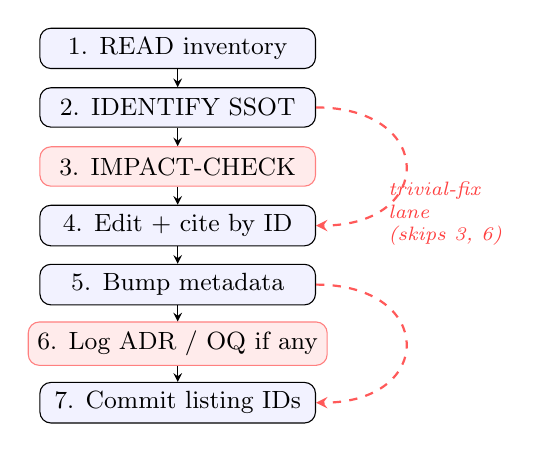
\begin{tikzpicture}[
    pstep/.style={draw,rounded corners,minimum width=3.5cm,minimum height=0.5cm,font=\small,fill=blue!5},
    skipbox/.style={draw,rounded corners,minimum width=3.5cm,minimum height=0.5cm,font=\small,fill=red!8,draw=red!50},
    arrow/.style={->,>=stealth},
    bypass/.style={->,>=stealth,red!65,dashed,thick},
]
\node[pstep]   (read)   at (0,5.6)  {1. READ inventory};
\node[pstep]   (id)     at (0,4.85) {2. IDENTIFY SSOT};
\node[skipbox] (impact) at (0,4.10) {3. IMPACT-CHECK};
\node[pstep]   (edit)   at (0,3.35) {4. Edit + cite by ID};
\node[pstep]   (bump)   at (0,2.60) {5. Bump metadata};
\node[skipbox] (decide) at (0,1.85) {6. Log ADR / OQ if any};
\node[pstep]   (commit) at (0,1.10) {7. Commit listing IDs};

% Main path (top-down through all steps)
\draw[arrow] (read)   -- (id);
\draw[arrow] (id)     -- (impact);
\draw[arrow] (impact) -- (edit);
\draw[arrow] (edit)   -- (bump);
\draw[arrow] (bump)   -- (decide);
\draw[arrow] (decide) -- (commit);

% Trivial-fix lane: red dashed bypasses skipping steps 3 and 6
\draw[bypass] (id.east)   to[out=0,in=0,looseness=2.6] (edit.east);
\draw[bypass] (bump.east) to[out=0,in=0,looseness=2.6] (commit.east);

% Annotation
\node[font=\scriptsize\itshape,red!75,anchor=west,align=left]
  at (2.55,3.5) {trivial-fix\\lane\\(skips 3, 6)};
\end{tikzpicture}
\caption{The edit protocol. The main path runs top-down through
all seven steps. The trivial-fix lane (red dashed arrows) bypasses
\textsc{impact-check} (step 3) and decision-logging (step 6),
which are the steps that do not apply to typos and
mechanical fixes. Steps 4, 5, and 7 always run.}
\label{fig:editproto}
\end{figure}

Before the edit: \textbf{READ} the inventory to confirm the artefact
exists at the expected status; \textbf{IDENTIFY} which artefact owns
the fact you intend to change (the Single Source of Truth, in the
language of \citet{hunt1999pragmatic}); and \textbf{IMPACT-CHECK} by
walking the artefact's \texttt{referenced\_by} list to identify
downstream artefacts that may need to update.

During the edit: touch the minimum surface needed. Use stable
identifiers in cross-references --- never file paths, never
paraphrases. Where you find yourself paraphrasing content from
another artefact, replace the paraphrase with a citation. Where you
find that the same fact lives in two artefacts, consolidate.

After the edit: bump \texttt{last\_reviewed}; if the change is
substantive, bump \texttt{version}; if status changes, update the
inventory in the same commit. If the edit reflects a decision among
alternatives, write the corresponding ADR in the same commit. If
the edit raises a question that cannot be resolved in line, write
the corresponding OQ. Commit messages list every artefact touched,
by stable identifier.

\paragraph{The trivial-fix lane.} A protocol that imposes the full
sequence on every typo is a protocol that gets bypassed. A
trivial-fix lane is built in: typos, formatting, broken markdown,
link fixes that do not change meaning skip the IMPACT-CHECK and the
decision-logging steps. The \texttt{last\_reviewed} field still
bumps. If you are uncertain whether a fix is trivial, it isn't; use
the full lane. The trivial lane exists to reduce extraneous
cognitive load \citep{sweller1988cognitive}, not to launder
ceremony around non-trivial changes.

\subsection{Forward and reverse propagation}

Changes at one layer of the abstraction hierarchy
(Figure~\ref{fig:hierarchy}) may imply work at others. The
discipline distinguishes two propagation directions.

\textbf{Forward propagation} is the high-to-low cascade. A change
to Requirements may flag downstream review of Design, Code, Tests,
and Operations. The discipline mandates that forward propagation
happen in the same commit if at all possible, or be filed as an
explicit OQ with a target resolution date if it cannot. A lurking
``I'll update the tests later'' is the road to drift.

\textbf{Reverse propagation} is the low-to-high direction.
Implementation may reveal a constraint not anticipated in design;
a test may surface a missing requirement; operations may reveal a
runtime constraint that requires architectural revision. The
discipline mandates that reverse propagation always pass through an
ADR. A higher-layer artefact is never silently retro-fitted to
match what was built; the ADR records that a lower-layer discovery
has caused a higher-layer revision.

A higher-layer artefact may be \emph{frozen} for a development
phase --- typically Requirements is frozen during implementation. A
frozen artefact is not edited; an ADR proposing the unfreeze is
required first. The protocol is heavy by design: opening
Requirements during implementation is exactly the kind of action
that benefits from deliberate friction.

The discipline of bidirectional propagation is what keeps the
hierarchy of abstraction layers more than a label. The layers
mean what they say only because changes to any layer cause review
of the others, and the reviews leave traces.

\subsection{Anti-patterns}

Most damaging mistakes recur. Naming them and forbidding them
explicitly is cheap insurance. The catalogue below is the
discipline's ``do not''.

\begin{enumerate}[nosep,leftmargin=1.2em]
\item Editing a \textsc{stable} artefact without bumping
  \texttt{last\_reviewed}. The change is invisible to the next
  reviewer.
\item Pasting the same content in two artefacts. A fact has one
  home.
\item Making a decision in conversation without writing the ADR.
  Phantom decisions are how this fails most.
\item Renaming an artefact's file without sweeping cross-references
  --- prevented by the stable-identifier convention if the
  identifier remains.
\item Creating an artefact without adding a row to the inventory.
  The artefact becomes an orphan no one will discover.
\item Quoting another artefact's prose verbatim. The duplicate will
  drift; the right move is a citation.
\item Letting Open Questions accumulate without target resolution
  dates. The OQ register becomes a wishlist instead of a register.
\item Mixing levels --- design specifics in Requirements, file
  paths in Design, configuration values in the Glossary. Each
  level has its language.
\item ``I'll update the tests later.'' The deferred propagation
  becomes the next session's drift.
\item Editing the body of a past ADR. Reversal goes through a
  superseding ADR; the past ADR is annotated with its supersession
  but otherwise immutable.
\item Bypassing the SSOT rule ``just for clarity''. Clarity is
  achieved through structure, not duplication.
\end{enumerate}

The catalogue is not exhaustive. New anti-patterns surface as the
discipline is practised in new domains; the catalogue grows
append-only.

\subsection{Session protocol}

The session-level discipline ensures every session begins by
reading the substrate and ends by depositing state back into it
(Figure~\ref{fig:session}). The substrate \emph{shadows} the problem
space at lower fidelity than full understanding but with
substantially higher stability (Figure~\ref{fig:substrate}).

% --- F7 Session Lifecycle ---
\begin{figure}[t]
\centering
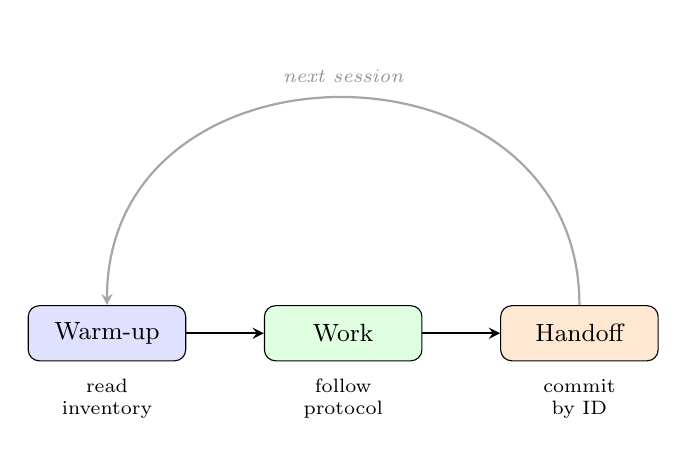
\begin{tikzpicture}[
    phase/.style={draw,rounded corners,minimum width=2.0cm,minimum height=0.7cm,font=\small},
    arrow/.style={->,>=stealth,thick},
]
\node[phase,fill=blue!12]   (warm) at (0,0.6) {Warm-up};
\node[phase,fill=green!12]  (work) at (3,0.6) {Work};
\node[phase,fill=orange!18] (hand) at (6,0.6) {Handoff};
\draw[arrow] (warm) -- (work);
\draw[arrow] (work) -- (hand);
% Loop back ABOVE the boxes (out=90,in=90) so it doesn't cross the descriptors below
\draw[arrow,gray!70,thick]
  (hand.north) to[out=90,in=90,looseness=1.5]
  node[above=2pt,font=\scriptsize\itshape,gray!85] {next session}
  (warm.north);
% Descriptors below each phase
\node[font=\scriptsize,below=0.1cm of warm,align=center] {read\\inventory};
\node[font=\scriptsize,below=0.1cm of work,align=center] {follow\\protocol};
\node[font=\scriptsize,below=0.1cm of hand,align=center] {commit\\by ID};
\end{tikzpicture}
\caption{Session lifecycle. Every session takes the same warm-up
path, whether the prior session ended cleanly or crashed. The
\emph{next session} loop is the same loop on every restart.}
\label{fig:session}
\end{figure}

% --- F8 Substrate Coverage ---
\begin{figure}[t]
\centering
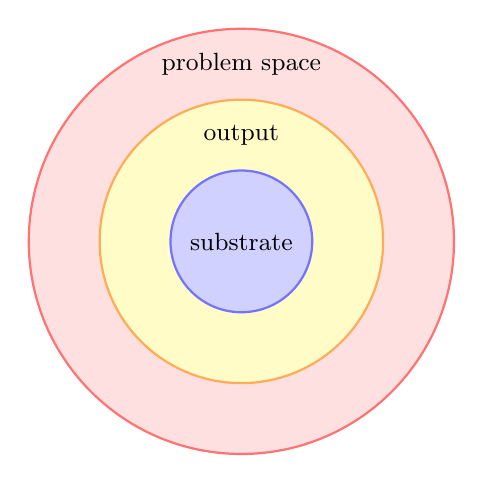
\begin{tikzpicture}
% \filldraw layers each draw stroke + fill cleanly; outer ring drawn first,
% inner rings drawn on top, so the labels in the inner bands sit on the
% appropriate fill.
\filldraw[fill=red!12,    draw=red!55,    thick] (0,0) circle (2.7);
\filldraw[fill=yellow!22, draw=orange!65, thick] (0,0) circle (1.8);
\filldraw[fill=blue!18,   draw=blue!55,   thick] (0,0) circle (0.9);
% Labels: each label sits in its own band, not on the centreline.
\node[font=\small] at (0,0)    {substrate};
\node[font=\small] at (0,1.35) {output};
\node[font=\small] at (0,2.25) {problem space};
\end{tikzpicture}
\caption{Substrate coverage. The substrate (inner disc, blue)
shadows the output ring (yellow) and the problem space (outer red)
at lower fidelity than full understanding, but with substantially
higher stability. Without a substrate, the output is fragile
against drift.}
\label{fig:substrate}
\end{figure}

\textbf{Warm-up.} Before any productive work in a new session: read
the inventory; read the protocol's TL;DR refresher; read the
artefacts the current task touches; spawn supplementary reads (or
explorer agents) for any unfamiliar dependencies. Five to ten
minutes spent on warm-up substantially reduces the rate of phantom
decisions, reference rot, and decided-versus-considered confusion
later in the session.

\textbf{Work.} Apply the edit protocol (\S4.4) to every change.
Cite artefacts by stable identifier in conversation, not by
paraphrase. Use task-tracking primitives to make multi-artefact
edits explicit and atomic. When in doubt about which artefact owns
a fact, stop and confirm before editing.

\textbf{Handoff.} Before declaring the session done: every edit is
committed; every new \textsc{missing} artefact created has a stub
frontmatter and an inventory row; every decision has its ADR;
every raised question has its OQ; \texttt{last\_reviewed} and
\texttt{version} are current on touched artefacts; the inventory's
priority queue reflects the new state. The next session's warm-up
is the previous session's handoff, read by whoever (or whatever)
is doing the next session.

The protocol applies symmetrically across the human and AI
collaborators. Both read the substrate at session start. Both
update it during work. Both leave it consistent at session end.
The asymmetry --- that the AI agent's session is bounded by its
context window in a way the human's is not --- is precisely what
the discipline is designed to compensate for.

% =====================================================================
\section{The Synthesis: Discipline $\leftrightarrow$ Cognitive Principle $\leftrightarrow$ Failure Mode}
\label{sec:synthesis}
% =====================================================================

This section is the paper's central synthesis. Each element of
Cognitive Cartography from \S\ref{sec:discipline} maps to a
cognitive principle from \S\ref{sec:foundations} that grounds it
and to a failure mode from \S\ref{sec:failures} that it mitigates.
Table~\ref{tab:synthesis} lays out the mapping.

% --- F6 Mapping Synthesis (table, full-width) ---
\begin{table*}[t]
\centering
\small
\begin{tabular}{p{4.4cm} p{5.7cm} p{5.4cm}}
\toprule
\textbf{Discipline element} & \textbf{Cognitive principle} & \textbf{Failure mode addressed} \\
\midrule
Hierarchy of abstraction layers & Marr's three levels of analysis \citep{marr1982vision}; hierarchical predictive coding \citep{clark2013whatever} & Drift across iterations; lost intent \\
Single Source of Truth + DRY-for-prose & External representations \citep{scaife1996external}; cognitive load \citep{sweller1988cognitive} & Decided-vs-considered confusion; reference rot \\
Stable identifiers (KB-N, ADR-N, OQ-N) & Boundary objects \citep{star1989boundary}; persistent symbolic anchors & Reference rot; phantom decisions \\
Append-only Decision Records & Distributed cognition \citep{hutchins1995}; preservation of reasoning trail & Phantom decisions; silent reversal \\
Status lifecycle (MISSING $\to$ DRAFT $\to$ STABLE $\to$ STALE) & Schema theory \citep{bartlett1932remembering}; affordances of state & Drift; stale knowledge \\
Edit protocol with trivial-fix lane & Cognitive load theory \citep{sweller1988cognitive}; chunking \citep{miller1956magical, cowan2001magical} & Restart cost; over-ceremony abandonment \\
Glossary as authoritative semantic anchor & Encoding specificity \citep{tulving1973encoding} & Terminology drift \\
Session warm-up + handoff protocol & Cognitive offloading \citep{risko2016offloading} & Restart cost; context-window saturation \\
\bottomrule
\end{tabular}
\caption{The synthesis. Each discipline element, the cognitive
principle that grounds it, and the failure mode (\S\ref{sec:failures})
it addresses.}
\label{tab:synthesis}
\end{table*}

The shape of the table matters as much as its content. Every
discipline element has a cognitive precedent, and every discipline
element addresses an observable failure. The discipline is not
arbitrary, and it is not a list of best practices. It is a small
set of structural choices, each with two sources of justification:
why it should work (the cognitive principle) and what happens when
it is absent (the failure mode).

Two readings of the table are useful. From left to right, it
answers ``why these elements?''. From right to left, it answers
``what to use against this failure?''. Both readings produce the
same set of correspondences. The redundancy is the synthesis's
robustness: every element is on the table for two independent
reasons.

A reader pressed for time should read \S1 and
Table~\ref{tab:synthesis}. The argument of the paper survives the
reduction.

% =====================================================================
\section{A Worked Example}
\label{sec:example}
% =====================================================================

We illustrate Cognitive Cartography with a single multi-month
project. Specifics are generalised: the project was a live
algorithmic-execution engine bridging a research backtesting
framework to a regulated broker. The engineering content of the
project is not the point. The point is the substrate trajectory.

The project began as a chat. A practitioner described the
problem: a backtesting framework that produces strategies, a broker
API to send them to live, the gap between the two. The first
artefact deposited to the substrate was a Requirements document ---
flat, around six thousand words, the practitioner's first pass at
what would be built and why.

The second artefact was a Context Inventory, listing the categories
of substrate the project would need: Knowledge Bases, Inventories,
Data Dictionaries, Decision Records, Open Questions, Glossary. The
inventory was at first largely \textsc{missing}; it named the
artefacts that would be needed without yet writing any.

The third artefact was a Context Protocol --- the discipline
document specifying how the substrate would be edited, how
cross-references would work, what the status lifecycle was. The
protocol came before most of the content because it determined how
the content would be added.

From there the substrate grew. The first Knowledge Base captured
the strategy taxonomy --- the archetypes the project would support.
That KB raised ten Open Questions about scope. The practitioner
made decisions on those OQs in a single working session; the
decisions became the project's first set of Architectural Decision
Records. The KB updated to mark the OQs as
\textsc{resolved-by-adr}; the OQs were not deleted, just
re-statused.

Knowledge Bases on the broker's API capabilities and pacing limits
followed. A Cost Dictionary on the project's cost models. A
Companion Projects map clarifying boundaries with related work. A
Frameworks Survey reviewing existing solutions and recording which
were adopted, studied, or rejected --- and why. Within a few
working sessions, thirteen Knowledge Bases existed; three
Inventories; nineteen Architectural Decision Records; twenty-two
Open Questions; one Glossary that had absorbed the terminology
sections of multiple other artefacts.

The Requirements document, originally a flat draft, underwent a
v0.2 pass: sections that had been narrative summaries of survey
content, decision rationale, and open questions were collapsed into
stable-identifier references to the relevant Knowledge Bases,
Architectural Decision Records, and Open Questions. The document
became substantially shorter, more authoritative, and easier to
update --- because the content it had been carrying now lived in
artefacts whose discipline was to be authoritative.

The substrate trajectory is the point. The project did not begin
with a plan and execute it. It began with the cheapest possible
substrate (a Requirements document) and grew the substrate as the
work demanded it, with the discipline ensuring that every growth
step left the artefact graph coherent. By the time implementation
began, the substrate was sufficient to absorb a session's worth of
work without drift, and the practitioner could resume after a break
of weeks without reconstruction cost.

The example does not prove the discipline works. It shows what the
discipline looks like in flight on a non-trivial project. The
metrics --- thirteen KBs, nineteen ADRs, twenty-two OQs --- are
incidental. The trajectory --- substrate as living artefact,
growing to match the project's demand for stability --- is the
substance.

% =====================================================================
\section{The Practice in the Hand}
\label{sec:practice}
% =====================================================================

Cognitive Cartography is not free. The discipline costs effort,
and the effort is borne by the practitioner. This section names
those costs honestly.

The protocol's heaviest cost is at the start. The first
substrate-disciplined session on a new project takes longer than
the same session run as flat chat, because the inventory is
\textsc{missing} and must be created, the protocol must be set up,
and the practitioner is doing two things at once: working on the
project, and building the substrate the project will live in.
This investment pays back roughly from session three or four,
when the substrate begins to absorb context that flat chat would
otherwise have demanded re-establish each session.

The ongoing cost is intrinsic load \citep{sweller1988cognitive}:
the discipline must be held in mind. The pre-edit READ, the
IDENTIFY SSOT, the IMPACT-CHECK --- none of these is hard, but
together they impose a small overhead on every change. The
trivial-fix lane absorbs much of the overhead for small changes;
the rest is amortised across the changes the discipline saves
elsewhere.

There is also a hidden requirement: someone must hold the substrate
in mind even while distributing it. The practitioner who maintains
a substrate at the level of discipline this paper specifies has
spent years building that capability across many projects, in
domains both AI-related and not. The discipline articulated here is
not Monday's lesson; it is the externalisation of years of internal
habit.

The threshold above which Cognitive Cartography pays back is
roughly: the project will span more than a handful of sessions,
or more than a handful of decisions of consequence, or more than
one collaborator. Below that threshold, flat chat and unstructured
notes are appropriate. Above it, every additional unit of
complexity exacerbates the failure modes of \S\ref{sec:failures}
and therefore widens the margin by which the discipline pays.

The discipline scales down naturally. Not every project needs
thirteen Knowledge Bases; some need three. Not every protocol
clause is invoked on every change; the trivial-fix lane is built
for the common case. The aim is not to maximise discipline; it is
to match discipline to project, with the project's complexity as
the dial.

% =====================================================================
\section{What Tooling Could Do for Cartographers}
\label{sec:tooling}
% =====================================================================

The discipline is practicable today with no special tooling --- a
text editor, a version-control system, and a project structure
suffice. But the discipline could be made substantially less
expensive with modest tooling support. We sketch the possibilities
here without proposing a system.

\textbf{Frontmatter validators.} An artefact's frontmatter
(\texttt{id}, \texttt{title}, \texttt{status}, \texttt{owner},
\texttt{last\_reviewed}, \texttt{version},
\texttt{depends\_on}, \texttt{referenced\_by}) is structured data.
A pre-commit hook can check that every artefact has frontmatter,
that the schema is correct, and that \texttt{last\_reviewed} is
more recent than the file's last modification time.

\textbf{Stable-identifier link checkers.} Every cross-reference is
of the form KB-N, ADR-N, OQ-N. A linter can confirm every
reference resolves to an existing artefact whose frontmatter
\texttt{id} matches.

\textbf{Inventory consistency.} The inventory of artefacts is
itself an artefact; an automated check should verify that every
file in the document tree has a row in the inventory, and every
row in the inventory has a file.

\textbf{Status-lifecycle automation.} A milestone-freeze gate
should be able to walk every \textsc{stable} artefact and check
its \texttt{last\_reviewed} date against the gate; artefacts that
haven't been reviewed by the gate should auto-degrade to
\textsc{stale}. The reverse --- promotion to \textsc{stable} ---
remains explicit, but degradation can be safely automatic.

\textbf{Session warm-up bundlers.} A tool that, given the
inventory and the current task, produces a recommended reading
list for session warm-up --- the artefacts in the task's
\texttt{depends\_on} closure, ordered by how recently each
changed. The human still reads; the tool just curates.

\textbf{Cross-reference graph visualisation.} The
\texttt{depends\_on} / \texttt{referenced\_by} graph is a navigable
structure. A static visualiser that produces a current picture of
the atlas (Figure~\ref{fig:atlas}) is mechanical and would replace
the hand-drawn diagram.

None of this is novel; all of it is specific application of
existing patterns (linters, schema validators, graph
visualisation). What is missing is a system that knows about
substrate as a first-class concept and supports the patterns
together. We do not build such a system here. We note that the
discipline does not require it. The system would be a force
multiplier; the discipline operates without it.

% =====================================================================
\section{Honest Costs and Limits}
\label{sec:limits}
% =====================================================================

A self-respecting methodology paper acknowledges where the
methodology fails. Cognitive Cartography is not universally
helpful. This section names where it doesn't help, where it costs
more than it returns, and where the assumptions break.

\textbf{Truly novel research.} The discipline assumes the project's
hierarchy of abstractions can be articulated. In genuinely novel
research --- where the right ontology is not known until the work
is mostly done --- the substrate cannot be designed in advance, and
forcing one is harmful. The discipline can be applied
retroactively, after the right structure has emerged, but it
cannot accelerate the emergence. For exploratory work, flat notes
are often better; substrate discipline applies once the work
crosses into elaboration.

\textbf{Bureaucracy risk.} A discipline whose ceremony exceeds its
benefit is a discipline that gets ignored or performatively
followed. The trivial-fix lane is built specifically to keep this
risk manageable, but the lane only works if it is generously sized.
A practitioner who narrows the trivial lane until every change
requires the full sequence will find their team --- or their agent
collaborator --- quietly bypassing the discipline. The discipline
must scale down or it scales out of relevance.

\textbf{Substrate-author expertise as hidden requirement.} A
substrate is no better than the discipline of its author. The
discipline articulated in this paper looks straightforward on the
page; in practice it requires judgement honed across many projects.
A practitioner attempting Cognitive Cartography for the first time
will produce a worse substrate than the same practitioner three
projects later. We have no way to shortcut this: the discipline is
teachable, but the judgement is practised.

\textbf{Multi-author coordination.} The discipline as specified
here assumes a single primary substrate author, with collaborators
(human and AI) operating against the substrate. Multiple authors
editing the substrate concurrently introduce coordination problems
--- branch-merge semantics, conflicting status changes, duplicate
ADRs --- that this paper does not address. The discipline extends
to multi-author settings, but the extension is its own work.

\textbf{The discipline is not a thinking aid.} Cognitive
Cartography helps a practitioner who has something to say organise
and sustain it. It does not generate ideas, evaluate alternatives,
or verify correctness. A well-organised wrong project is still
wrong. The discipline preserves the practitioner's reasoning; it
does not produce it.

\textbf{Model capability still matters.} We have argued that
substrate matters as much as model. We have not argued that model
capability is irrelevant. A model that cannot follow instructions,
cite stable identifiers, or refrain from hallucinating in spite of
contradicting evidence cannot be a useful collaborator on a
disciplined substrate. Substrate amplifies model capability; it
does not replace it.

These caveats do not invalidate the discipline. They locate it.
Cognitive Cartography is the right tool for sustained complex
work with a capable AI collaborator, above a complexity threshold,
where the project's structure is articulable. Outside that
envelope it costs more than it returns, and we do not recommend
it.

% =====================================================================
\section{A Cognitive Practice for the AI Era}
\label{sec:close}
% =====================================================================

We close on the deepest implication.

AI raises the importance of work humans have always needed to do.
Externalising thought, structuring it hierarchically, preserving
reasoning trails, naming things stably --- none of this is new.
Books, libraries, encyclopedias, scientific notation, version
control, lab notebooks, architectural decision records: every
generation has produced apparatus for stabilising thought across
time and distributing it across minds. The apparatus has worked.

What is new is the collaborator. A large language model is the
first collaborator with the cognitive capacity of a careful
specialist and the persistent memory of a goldfish. The asymmetry
is unique: any session begins with the agent's full intelligence
intact and the project's accumulated context absent. Substrate is
how the absence is repaired, every session, indefinitely.

The discipline that addresses this is not invented for it. The
discipline is recovered, from cognitive science, from
software-engineering, and from agentic-AI literatures, and made
explicit. The practice is fundamentally human: a person cultivates
it, with AI as participant. AI's limitations motivate it; human
practice executes it. The practice survives across model
generations because it is about how minds collaborate on complex
problems, not about which model is current.

Substrate is the leverage point currently most under-practised in
AI work. Model capability per token will continue to grow, and
context windows will continue to lengthen, and benchmarks will
continue to shift. None of this changes the substrate problem. The
complexity of any project that matters grows faster than any
plausible future model can absorb in a single context. The
projects that succeed will be the ones whose substrate keeps pace.

Cognitive Cartography is one form of the practice. There may be
others. What matters is that the practice exists, that it is
explicit, that it is taught, and that it is shared. We have
described one form. We expect the form to evolve. The form's
evolution is itself a forward-propagation event the discipline
foresees.

% =====================================================================
\section*{Acknowledgements}
% =====================================================================

The discipline articulated in this paper is the author's, cultivated
across many disciplines and projects over years of sustained complex
work, of which collaboration with current-generation AI agents is
the most recent and most demanding instance --- not its origin. The
discipline's choices --- its artefact categories, the status
lifecycle, the edit protocol, the propagation rules, and the
discipline's overall shape --- were practised and refined long
before they were named here. Anthropic's Claude provided substantial
assistance in drafting and stress-testing the articulation in this
paper, particularly in tracing precedents in the cognitive-science
and software-engineering literatures and in helping render implicit
practice into explicit specification. The writing was a
collaboration in the spirit the paper itself describes; the
discipline it articulates was not.

% =====================================================================
% References
% =====================================================================
\bibliographystyle{plainnat}
\bibliography{references}

% =====================================================================
\appendix
% =====================================================================

\section{The Cartographer's Compact Field Manual}
\label{app:manual}

This appendix collects the discipline in a form a practitioner can
print and pin. Repetition is by design: the protocol's steps are
short enough that the appendix should be readable on its own.

\subsection*{Frontmatter (every artefact)}

\begin{verbatim}
---
id: KB-NNN | INV-NNN | DD-NNN
    | ADR-NNN | OQ-NNN
title: human-readable title
status: MISSING | DRAFT | STABLE
       | STALE | DEPRECATED
owner: Name | shared
last_reviewed: YYYY-MM-DD
version: 0.1
sources: [URLs with date accessed]
depends_on: [ID, ID, ...]
referenced_by: [ID, ID, ...]
---
\end{verbatim}

\subsection*{Edit protocol (every non-trivial change)}

\begin{enumerate}[nosep,leftmargin=1.2em]
\item READ the inventory; locate the artefact.
\item READ its frontmatter.
\item IDENTIFY the SSOT for the fact you intend to change.
\item IMPACT-CHECK by walking \texttt{referenced\_by}.
\item Decide the lane: trivial / normal / decision-bearing.
\item Edit; cite by stable identifier; do not restate.
\item Bump \texttt{last\_reviewed}; bump \texttt{version} if substantive.
\item Update inventory if status changed.
\item Log decision as ADR if applicable.
\item Log question as OQ if applicable.
\item Commit; commit message lists every artefact touched, by ID.
\end{enumerate}

\subsection*{Trivial-fix lane}

For typos, formatting, broken links that do not change meaning:
skip steps 4, 9, 10. Still bump \texttt{last\_reviewed}. If unsure
whether a fix is trivial, it isn't; use the full lane.

\subsection*{Status transitions}

\begin{itemize}[nosep,leftmargin=1.2em]
\item \textsc{missing} $\to$ \textsc{draft}: first content commit.
\item \textsc{draft} $\to$ \textsc{stable}: owner review; complete; no \textsc{todo}.
\item \textsc{stable} $\to$ \textsc{stale}: \texttt{last\_reviewed} older than current milestone freeze, or upstream changed.
\item \textsc{stale} $\to$ \textsc{stable}: re-review.
\item Any $\to$ \textsc{deprecated}: superseded.
\end{itemize}

\subsection*{Anti-patterns (do not)}

\begin{enumerate}[nosep,leftmargin=1.2em]
\item Edit \textsc{stable} without bumping \texttt{last\_reviewed}.
\item Paste the same content in two artefacts.
\item Decide in conversation without an ADR.
\item Create an artefact without an inventory row.
\item Quote another artefact's prose verbatim.
\item Let OQs accumulate without target dates.
\item Mix levels of abstraction in one artefact.
\item Defer propagation (``I'll update tests later'').
\item Edit a past ADR's body.
\item Bypass SSOT ``just for clarity''.
\end{enumerate}

\subsection*{Session protocol}

\textbf{Warm-up.} Read inventory; read protocol TL;DR; read task's
artefacts; spawn supplementary reads.

\textbf{Work.} Apply edit protocol; cite by ID; track multi-artefact
edits as a unit.

\textbf{Handoff.} Every edit committed; every new artefact has
frontmatter and inventory row; decisions in ADRs; questions in OQs;
metadata current; inventory's priority queue reflects new state.

\end{document}
